\documentclass[12pt]{article}

\usepackage{sbc-template}

\usepackage{graphicx,url}

\usepackage[brazil]{babel}   
  
\usepackage[utf8]{inputenc}  

     
\sloppy

\title{Usando simuladores para entender predição de desvio}
\author{Rafael Rodrigues dos Santos\inst{1}, Thais Aparecida Silva Camacho\inst{1}}

\address{
  Departamento de Informática\\
  Universidade Estadual de Maringá -- Maringá, PR -- Brazil
  \email{rafael11rodrigues@hotmail.com, thaiscamachoo@gmail.com}
}


\begin{document} 

\maketitle

\section{Introdução}

O uso de simuladores é uma grande ferramenta de ensino e pesquisa. Eles permitem aplicar na prática os conhecimentos adquiridos nos estudos, obtendo-se uma
melhor compreensão do conteúdo teórico.

O conjunto de ferramentas SimpleScalar \cite{austin1997user} permite simular um processador superescalar com diversos graus de complexidade, podendo especificar
estrutura de caches, acesso à memória, tipos de previsores de desvios entre outras funcionalidades. Tais ferramentas podem ser utilizadas para melhor
entendimento sobre arquiteturas superescalares e o pipeline.

O objetivo deste artigo é descrever nossas simulações no SimpleScalar, utilizando-se dos programas de testes da estrutura LLVM (Test Suite), com enfoque nas técnicas de predição de desvio.

\section{Fundamentação Teórica} \label{sec:firstpage} 

\subsection{SimpleScalar}

O SimpleScalar foi desenvolvido na Universidade de Wisconsin-Madison sob a coordenação de Gurindar S. Sohi e posteriormente Doug Burger disponibilizou uma versão gratuita do simulador para uso não comercial. Para manter a portabilidade entre vários sistemas, tal simulador possui duas versões, big-endian e little-endian. 

A ferramenta de simulação SimpleScalar é constituída por um conjunto de vários simuladores, os quais estão listados na tabela \ref{tab:tblsimulador}. Dessa
forma, o SimpleScalar pode viabilizar simulações de arquiteturas de forma rápida e concisa através do sim-fast ou simulações mais detalhadas e dinâmicas através
do sim-outorder; diversas técnicas de predição de desvio; execução especulativa e renomeação de registradores.

\begin{table}[ht]
\centering
\caption{Simuladores do SimpleScalar}
\label{tab:tblsimulador}
\smallskip
\begin{tabular}{l|l}
\hline
\textbf{Simulador} & \textbf{Descrição} \\[0.5ex]
\hline
sim-safe & Simulador simples\\[0.5ex]
\hline
sim-fast & Simulador otimizado \\[0.5ex]
\hline
sim-profile & Programa dinâmico para análise \\[0.5ex]
\hline
sim-bpred & Simulador de previsão de desvios \\[0.5ex]
\hline
sim-cache & Simulador de caches multiníveis \\[0.5ex]
\hline
sim-outorder & Simulador de microarquiteturas detalhado \\[0.5ex]
\hline
\end{tabular}
\end{table}

O SimpleScalar pode simular tanto a semântica do conjunto de instruções (ISA) PISA (Portable Instruction Set Architecture) como o conjunto de instruções Alpha. O conjunto de instruções PISA é um conjunto de instruções MIPS simples.

\subsubsection{Sim-Bpred}

O Sim-Bpred é um simulador de preditores de desvio e tem como função principal o teste de desempenho de preditores estáticos e dinâmicos. Tal simulador
implementa duas técnicas de predição de desvio estática (taken e nottaken) e três dinâmicas (bimodal, 2 níveis e combinado). O conjunto de parâmetros de
controle de entrada do Sim-Bpred é apresentado na tabela \ref{tab:tblsimuladorp}.


\begin{table}[ht]
\centering
\caption{Parâmetros de Controle de Entrada dos Simuladores do SimpleScalar}
\label{tab:tblsimuladorp}
\smallskip
\begin{tabular}{l|l}
\hline
\textbf{Parâmetros} & \textbf{Detalhes} \\[0.5ex]
\hline
-config & configurar o simulador via arquivo externo \\[0.5ex]
\hline
-h & mostrar opções de ajuda na tela \\[0.5ex]
\hline
-d & habilitar mensagem de debug \\[0.5ex]
\hline
-redir:sim & redirecionar saída de simulação \\[0.5ex]
\hline
-redir:prog & redirecionar saída do programa \\[0.5ex]
\hline
-max:inst & limitar o número de instruções testadas \\[0.5ex]
\hline
-bpred & escolher uma técnica especifica de predição de desvio \\[0.5ex]
\hline
\end{tabular}
\end{table}

\subsection{LLVM Teste Suite}

A infraestrutura de testes LLVM contém duas principais categorias de teste: Regression Tests e Teste Suite. A Regression Tests é composta por pequenos pedações de código que testam uma característica específica ou desencadeiam um bug específico no LLVM.

Já a categoria Teste Suite é composta por pedaços de código que podem ser compiladas e vinculadas em um programa autônomo que pode ser executado. A LLVM Teste Suite é organizada em

\begin{itemize}
	\item SingleSource (Pequenos Benchmarks)
	\item MultiSource (Grandes Benchmarks)
	\item External (Parecido com o SPEC Benchmarks)
\end{itemize}

\section{Experimentos e Discuções}

Os programas escolhidos para os experimentos foram o heapsort e o matrix, pertencentes a categoria SingleSource. Para as simulações foi utilizado no SimpleScalar o conjunto de instruções PISA e a análise foi realizada em cima dos preditores estáticos taken e nottaken; e os preditores dinâmicos contadores saturados (bimod), em 2 níveis (2lev) e híbridos (comb).

A escolha de tais programas foi embasada na estrutura do código deles, pois enquanto o código do matrix é marcado por vários loops e chamadas de funções, o
código do heapsort é marcado por estruturas IF-THEN-ELSE para a comparação dos números aleatórios a serem ordenados. Os loops são saltos condicionais quase
sempre tomados (apenas o salto após a última iteração não é tomado); chamadas de funções são saltos incondicionais (que sempre são tomados); estruturas IF-THEN-ELSE são saltos condicionais sem um padrão de comportamento como o dos loops e têm forte relação com os dados de entrada. Logo, os dois programas escolhidos
permitem analisar situações bastante diferentes.

Os programas escolhidos apresentaram grande diferença nos testes realizados, começando pela porcentagem das classes de instruções executadas.
O programa matrix teve mais de 6 vezes a quantidade de desvios incondicionais e quase 4 vezes a quantidade de desvios condicionais executados pelo heapsort,  como pode ser observado na figura \ref{fig:classes}.

\begin{figure}[ht]
\centering
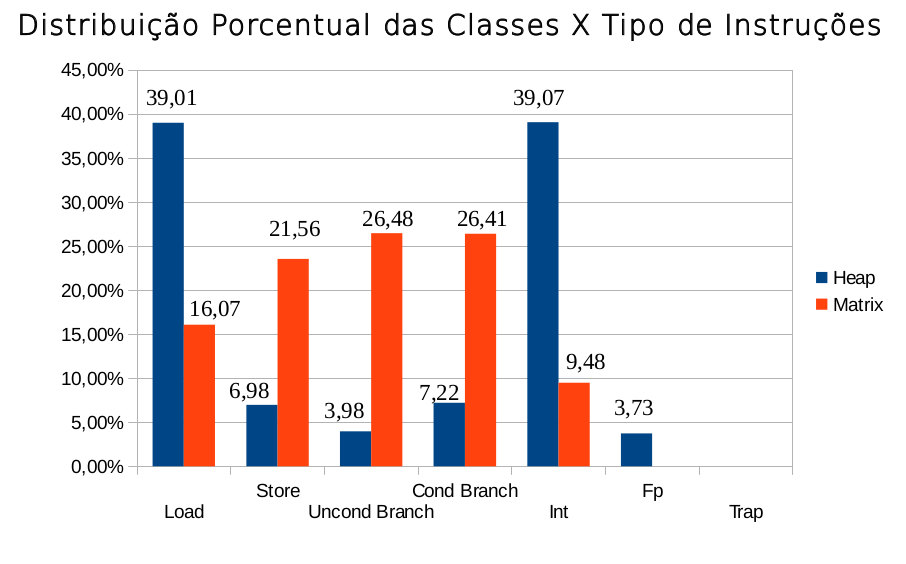
\includegraphics[width=.8\textwidth]{graf11.png}
\caption{Perfis das classes de instruções do HeapSort e Matrix.}
\label{fig:classes}
\end{figure}

Essa diferença se deve ao fato do matrix ter muitos loops e chamadas de funções. Tal observação será importante nos resultados referentes a predição de desvio,
que serão apresentados mais adiante.

Na simulação realizada no Sim-Bpred para cada técnica de predição de desvio obteve-se as taxas de misses representadas na figura \ref{fig:sim-bpred}. É possível
notar que o heapsort possui como melhor preditor em termos de acertos o preditor dinâmico 2lev com 90,93\% de acertos. Já o matrix teve como maior taxa de
acertos 95,46\%, obtida pelo preditor estático taken, com uma diferença mínima entre os preditores dinâmicos que obteram taxas iguais de 95,42\%.

\begin{figure}[ht]
\centering
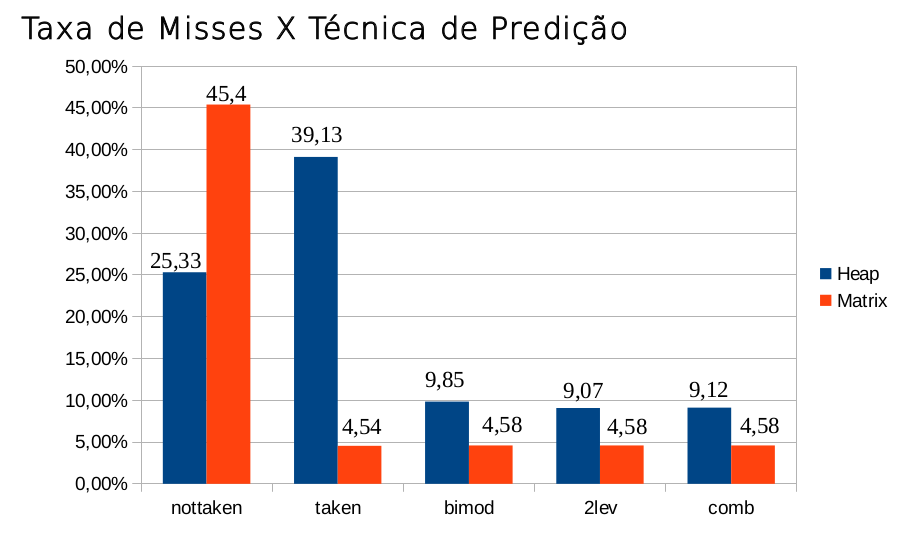
\includegraphics[width=.8\textwidth]{graf22.png}
\caption{Taxa de misses em função das técnicas de predição de desvio do HeapSort e do Matrix.}
\label{fig:sim-bpred}
\end{figure}

Tais resultados mostram que a taxa de acertos de um preditor é muito influenciada pela estrutura do código, pois apesar das técnicas de predisão dinâmica se
basearem no histórico de execução e por supostamente acertarem mais que as técnicas de predisão estática.
Pelo fato dos desvios do matrix serem oriundos de loops, chamadas e retornos de função que, como já mencionado, são desvios sempre tomados, a técnica taken foi a com maior taxa de acerto.

Dessa forma, na técnica taken o programa heapsort pode ser considerado como ``ruim'' e o matrix como ``bom'', pois a taxa de misses do matrix foi de 4,58\%,
enquanto que no heapsort a taxa de misses foi quase 40\%. Tal fato acontece pois, como já mencionado, os desvios do matrix se deve a desvios relacionados a
loop, chamada e retorno de subrotinas. Diferente do heapsort, que a grande parte dos desvios são oriundos da estrutura IF-THEN-ELSE, que têm um comportamento
mais ``aleatório''.

Observa-se ainda que em todas as técnicas, menos na nottaken, o matrix obteve baixa taxa de misses, e mais, as taxas dele ficaram abaixo das taxas do heapsort.
Ou seja, mesmo o matrix tendo mais desvio do que o heapsort, ele obteve na maioria das técnicas simuladas menor taxa de misses. Isto ocorre, pois os desvios do heapsort oriundos da estrutura IF-THEN-ELSE são díficeis de prever, já que são comparações de números aleatórios.

Em ambos os programas, mesmo as estruturas deles serem bem diferentes, as técnicas dinâmicas se mostraram eficientes como já esperado. Já na técnica nottaken, ambos foram ``ruins'', com a taxa de misses do matrix bem maior que a do heapsort, já que a maioria dos desvios do matrix são os famosos desvios ``sempre tomados''.

Para uma análise mais concreta do desempenho dos preditores de desvio, realizou-se as simulações do heapsort no Sim-Outorder.  No simulador Sim-Outorder, além dos 5 preditores anteriores pode-se utilizar o preditor perfeito (perfect). Tal simulador testa as funcionalidades e o desempenho da configuração simulado, comparando ao preditor perfeito. Como o preditor perfeito acerta todas as previsões, não faz sentido testar funcionalidade de um preditor de desvio que acerta todas as predições no Sim-Bpred, pois ele é um simulador funcional.

O desempenho do heapsort pode ser verificado na tabela \ref{tab:tblheap}. Nota-se que, à medida que o tipo de preditor acerta mais as predições, o número de
instruções por ciclo (IPC) aumenta proporcionalmente, sendo o limite superior o preditor perfeito. Consequentemente, sendo o limite inferior o preditor perfeito,  o número de ciclos por instrução (CPI) diminui também proporcionalmente. Ou seja, quanto maior a taxa de acerto do preditor de desvio, tem-se um desempenho maior do processador.

\begin{table}[ht]
\centering
\caption{Métricas em função da técnica de predição de desvio do heapsort.}
\label{tab:tblheap}
\smallskip
\begin{tabular}{l|l|l|l|l|l|l}
\hline
\textbf{Heapsort} & \textbf{taken} & \textbf{nottaken} & \textbf{2lev} & \textbf{comb} & \textbf{bimod} & \textbf{perfect} \\[0.5ex]
\hline
hits \% & 60,47 & 60,47 & 91,47 & 91,48 & 90,979 & 100 \\[0.5ex]
\hline
IPC & 0,8800 & 0,8799 & 1,2331 & 1,2365 & 1,2283 & 1,3856 \\[0.5ex]
\hline
CPI & 1,1364 & 1,1365 & 0,8109 & 0,8087 & 0,8142 & 0,7217 \\[0.5ex]
\hline
razão \% & 63,51 & 63,50 & 88,99 & 89,23 & 88,64 & 100 \\[0.5ex]
\hline
\end{tabular} \\
razão = (100*IPC preditor análisado)/IPC do preditor perfeito
\end{table}

Também foi percebido que, a análise das razões do heapsort favorece a predição com técnica combinada, pela proximidade com a ideal (89,23\%) e pela taxa de predições
certas (90,75\%), demonstrando desta forma, ser o modo mais eficiente para o heapsort.

\section{Conclusão}

O uso do SimpleScalar foi um grande facilitador para o estudo das técnicas de predição de desvio, permitindo a validação do conhecimento teórico na prática.

Para as simulações, o simulador Sim-Bpred mostrou-se eficiente, mas para um entendimento mais detalhado foi-se necessário a realização de simulações no Sim-Profile e no Sim-Outorder. O Sim-Profile contribuiu com a identificação das classes de instruções envolvidas em cada programa e o Sim-Outorder deu uma visão do desempenho de cada preditor de desvio com o preditor perfeito, permitindo analisar qual preditor chegou mais próximo do ideal.

Para a análise o enfoque principal foi na relação dos resultados de cada técnica de predição de desvio com o código de cada programa, pensando também no aumento do desempenho para o processador nos resultados obtidos no IPC e CPI. Validando a importância de se ter técnicas de predição de desvio eficientes, pois foi observado como a taxa de acerto reflete no IPC e no CPI. 

Neste artigo, as simulações foram conduzidas com o objetivo de entendimento e validação das técnicas de predição de desvio, mas com o SimpleScalar pode-se realizar simulações para a visão global de projeto de processadores. 

\nocite{austin2002simplescalar}
\nocite{simple}
\nocite{analise}

\bibliographystyle{sbc}
\bibliography{referencias}

\end{document}